\chapter{State of the Art}
\label{chap:soa}

In this chapter, we discuss the current state of the art in knowledge graph construction using declarative mapping rules. We provide an overview of approaches, techniques and methodologies for constructing and querying (virtual) knowledge graphs based on semantic technologies. We describe the declarative annotations and mapping languages specifications that have been proposed to construct these kind of data models together with their main features. We also present the current methodologies to evaluate the quality of knowledge graph construction engines such as benchmarkings and test-cases. 

More in detail, in Section \ref{sec:soa_integration} we describe the foundations of data integration concept and its relation with the theoretical contributions where the global schema is defined by an ontology. Section \ref{sec:soa_representation} summarizes the languages used for representing and querying data on the Semantic Web (i.e., the RDF model and the SPARQL query language). Section \ref{sec:soa_annotations} presents an overview of the most important contributions for representing declarative annotations with a focus on the representations of mapping rules and data constraints. Additionally, Section \ref{sec:soa_engines} describes the most relevant knowledge graph construction systems and their corresponding optimizations while Section \ref{sec:soa_evaluations} finally, describes evaluation methodologies used for these approaches. We conclude in Section \ref{sec:soa_conclusions} with a summary and conclusions on the current gaps, which will help to understand the contributions of this thesis.


\section{Data Integration and OBDA}
\label{sec:soa_integration}
A data integration system (DIS) is defined as the process of making available a set of different sources through a common view~\citep{Lenzerini02}. Formally, it is described as $DIS$ = $\langle \mathcal{G}, \mathcal{S}, \mathcal{M} \rangle$, where:
\begin{itemize}
    \item $\mathcal{G}$ is the \textit{global schema}, expressed in a language $\mathcal{L_G}$ over an alphabet $\mathcal{A_G}$.
    
    \item $\mathcal{S}$ is the \textit{source schema}, expressed in a language $\mathcal{L_S}$ over an alphabet $\mathcal{A_S}$.
    
    \item $\mathcal{M}$ is the \textit{mapping} between $\mathcal{G}$ and $\mathcal{S}$, constituted by a set of assertions matching queries over $\mathcal{S}$ and $\mathcal{G}$, in order to establish correspondences between concepts in both schemes.
\end{itemize}

Different types of data integration systems have been proposed in the literature and are applied in research and data scenarios. Data warehouses~\citep{vassiliadis2009survey} are proposed to integrate multiple and heterogeneous data sources in a centralized storage system. The process of feeding such system with data is usually known in enterprises ecosystems as an \textit{extract-transform-load} process (ETL). In contrast, mediators~\citep{wiederhold1992mediators} have been proposed as another data integration approach where the data remains in the data sources. For accessing the data, queries defined over the global schema are translated to the source schema and executed. Multiple systems that implement these ideas with their corresponding optimizations~\citep{tsimmis1994,rajaraman1996querying,roth1997don}.

Ontology based data access (OBDA) and integration (OBDI) are data integration systems where the global schema is defined by an ontology~\citep{poggi2008linking}. The formal framework presented in~\citep{xiao2018obdasurvey} defines an OBDA specification as a tuple $P$ = $\langle O,S,M\rangle$ where $O$ is an ontology, $S$ is the source schema, and $M$ a set of mappings. Additionally, an OBDA instance is defined as a tuple $PI$ = $\langle P,D\rangle$ where P is an OBDA specification and $D$ is a data instance conforming to $S$. The main difference between OBDA and OBDI systems is that in OBDA $D$ is fixed to a single data source in a specific data format, while OBDI extends $D$ to cover heterogeneous data sources and formats. In both ontology-based approaches, two different alternatives exist to enable data access: (1) those where data are materialized taking into account the mappings and the ontologies, what can be seen as a ontology-based ETL process, and (2) those where the transformation is done on the queries, which can then be evaluated on the original data sources, so, it can be defined as a kind of mediator system. In this work we refer to the first alternative as a materialized knowledge graph construction process, while the second alternative is defined as a virtual knowledge graph construction one. As we are focused on creating KG from heterogeneous data sources, both alternatives can be described as an OBDI approach.

\section{Representation and Query Languages for the Semantic Web}
\label{sec:soa_representation}
In this section, we provide an overview of the core semantic web languages that have a relevant role during a knowledge graph construction process. We discuss in detail the Resource Description Framework (RDF)~\citep{RDF}, used for implementing the target data model in the DIS (i.e., the ontology), but also usually used for declaring mapping rules~\citep{R2RML,dimou2014rml,michel2015translation}. We also provide a detailed explanation of the SPARQL query language~\citep{SPARQL} as it is an essential input for virtual knowledge graph construction techniques (e.g., translating SPARQL to SQL).

\subsection{RDF: Resource Description Framework}
The Resource Description Framework (RDF)~\citep{RDF} is the basic data model used in the Semantic Web. Basically, RDF is defined by a set of \textit{triples}, where each triple is represented in the form of $<s,p,o>$ where $s$ is the subject, $p$ the predicate and $o$ the object. One of the main features of RDF is the used of IRIs to represent concepts and the relationships between them. This allows having unique identifiers across the Web for each resource. Assuming that there are a pairwise disjoint infinite $I$, $B$ and $L$ (IRIs, blank nodes and literals respectively), we can formally defined an RDF triple as $(s,p,o) \in (I \cup B) \times I \times (I \cup B \cup L)$~\citep{perez2009semantics}. Additionally, we can define $G$ as an RDF graph composed by a set of RDF triples.

Listing \ref{list:soa_rdf_example} shows an example of an RDF graph with a set of triples in the transport domain (shown in its graphical representation in Figure \ref{fig:soa_rdf_example}). As we can observe, there are, in total, 4 different triples (or statements), all of them with the same subject, defined using the URI \textit{http://example.org/transport/trip/1}. We can also observe that all the predicates of the triples (e.g., http://vocab.gtfs.org/terms\#stop) are also defined by an IRI. More in detail, the first triple declares that \textit{http://example.org/transport/trip/1} is a trip defined in the LinkedGTFS vocabulary\footnote{\url{http://vocab.gtfs.org/terms}}. The predicate \texttt{rdf:type} is used in the RDF data model for classify the resources. Then, predicates \texttt{gtfs:shortName} and \texttt{gtfs:wheelchair} represent the information about the name of the trip and if it is accessible or not using a wheelchair. The objects of these two triples are literals in RDF that can be either simple string (``Puerta del Sur'') or typed literal (``false''$\hat{\;}\hat{\;}$xsd:boolean). The typed literals contain data values with a tag for representing its data type. Finally, \texttt{gtfs:stop} indicates one of the trips stops, using and IRI, which means that the stop is also a resource. 


\begin{lstlisting}[float,caption=Example of RDF graph,frame=tlrb,label={list:soa_rdf_example}, columns=fullflexible]
@prefix gtfs: <http://vocab.gtfs.org/terms#> .
@prefix xsd: <http://www.w3.org/2001/XMLSchema#> .

<http://example.org/trip/1> rdf:type gtfs:Trip .
<http://example.org/trip/1> gtfs:stop <http://transport.org/stop/360> .
<http://example.org/trip/1> gtfs:shortName "Puerta del Sur" .
<http://example.org/trip/1> gtfs:wheelchair "false"^^xsd:boolean .
\end{lstlisting}

\begin{figure}[!ht]
\centering
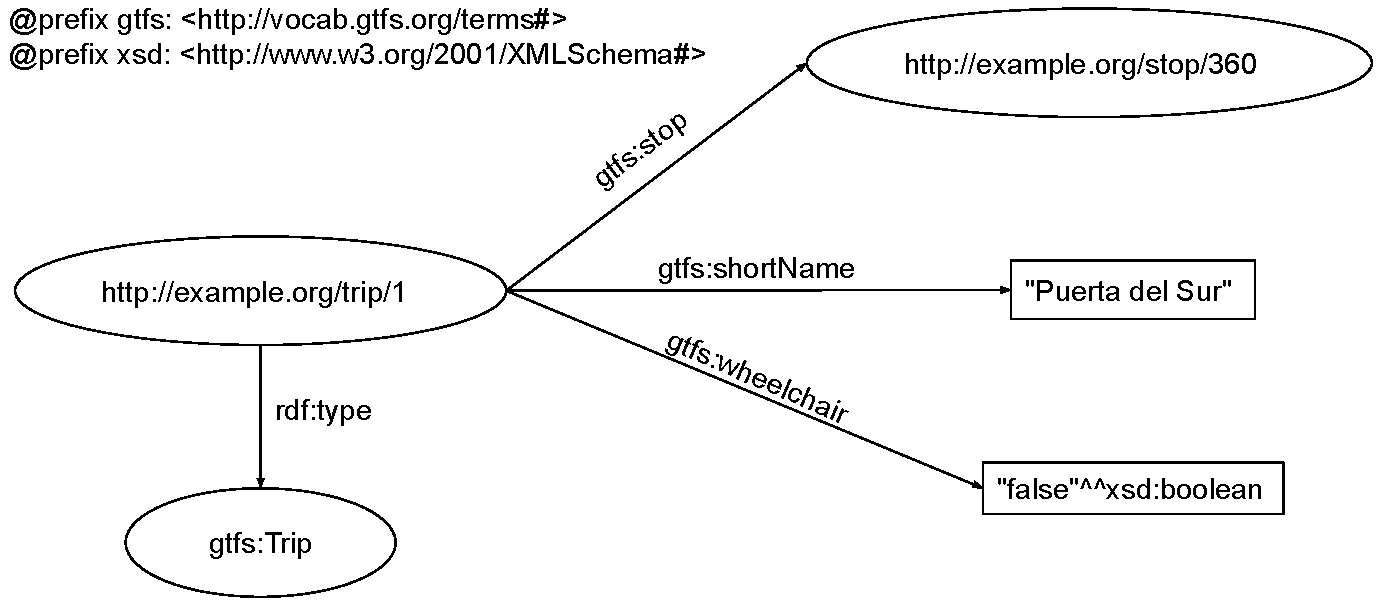
\includegraphics[width=\textwidth]{figures/state-of-the-art/RDF.pdf}
\caption{Graphical representation of an RDF Graph}
\label{fig:soa_rdf_example}
\end{figure}


Several formats can be used to serialize an RDF graph. RDF/XML\footnote{\url{https://www.w3.org/TR/rdf-syntax-grammar/}} was the first serialization to be proposed and it is supported by XML. Notation 3 (N3) provides a human readable serialization, although currently is not used widely. N-Triples\footnote{\url{https://www.w3.org/TR/n-triples/}} and Turtle\footnote{\url{https://www.w3.org/TR/turtle/}} are subsets of N3, more widely adopted. Finally, the last serialization that has been proposed as W3C recommendation is JSON-LD\footnote{\url{https://www.w3.org/TR/json-ld11/}}. Since it is based on JSON, it facilitates the consumption of RDF data to developers and practitioners as it encapsulates the RDF in a standard JSON document. There are other serialization of RDF that are not recommended by W3C but are highly adopted for specific purposes. For example, HDT~\citep{fernandez2013binary} is a binary serialization of RDF for publishing and exchanging RDF data at large scale.

\begin{lstlisting}[float,caption=Example of SPARQL query,frame=tlrb,label={list:soa_sparql_example}, columns=fullflexible]
PREFIX gtfs: <http://vocab.gtfs.org/terms#> .

SELECT ?name WHERE {
    ?trip rdf:type gtfs:Trip .
    ?trip gtfs:shortName ?name .
}
\end{lstlisting}
\subsection{SPARQL}
SPARQL is the W3C recommendation graph matching query language for RDF graphs. For defining the syntax of the query language we use the work presented in~\citep{perez2009semantics}, which defines the SPARQL graph patterns recursively as follows:
\begin{itemize}
    \item A tuple $(I \cup V) \times (I \cup V) \times (I \cup L \cup V)$ is a graph pattern (triple pattern if it is single), where $I$ is an IRI, $V$ is a variable and $L$ a literal.
    \item If $P_1$ and $P_2$ are graph patterns, then expression ($P_1$ AND $P_2$), ($P_1$ OPT $P_2$) and ($P_1$ UNION $P_2$) are also graph patterns.
    \item If $P$ is a graph pattern and $R$ is a SPARQL built-in condition, then ($P$ FILTER $R$) is also a graph pattern.
    \item If $P$ is a graph pattern and $T$ is a finite set of variables, then (SELECT $T$ WHERE $P$) is a graph pattern.
\end{itemize}

Given the RDF graph shown in Figure \ref{fig:soa_rdf_example}, we may be interested in obtained the name of the trips of our graph. In Listing \ref{list:soa_sparql_example} we depict the SPARQL query used for obtaining the desirable result-set. The first part of the query defines the prefixes that can be used in the query. Then, the SELECT operator indicates the set of variables that will be projected from the graph pattern in query result-set (?name). Variables in SPARQL are represented using the question mark before the variable name (in the example ?name or ?trip are variables). During the query evaluation process, the variables are bound to the different values of the RDF graph that match with the triples pattern (formal definition described in~\citep{perez2009semantics}). In the example, the variable ?trip is bound to \textit{http://transport.org/trip/1 } as there are two facts in the graph that match with the two triple patterns defined in the query. Then, variable ?name is bound to ``Puerta del Sur'' and retrieved in the SPARQL result-set, usually represented in the form of a table where each column contains the values of each projected variable (see Table \ref{tab:soa_result_set}).




% Please add the following required packages to your document preamble:
% \usepackage{graphicx}
\begin{table}[!ht]
\centering
\caption{Example of a SPARQL result-set}
\label{tab:soa_result_set}
\resizebox{0.2\textwidth}{!}{%
\begin{tabular}{|c|}
\hline
\textbf{?name} \\ \hline
``Puerta del Sur'' \\ \hline
\end{tabular}%
}
\end{table}

The SPARQL built-in conditions are constructed using the elements of the set ($I \cup U$) and constants. These constants can take different values such as logical connectives ($\neg,\wedge,\vee $), inequality or equality symbols ($\leq,\geq,<,>,= $) and unary predicates such as bound, isBlank, isIRI, etc.~\citep{SPARQL}. The can be combined with the aforementioned SPARQL operator such as UNION, FILTER or OPTIONAL. For example, the OPTIONAL operator attracted much attention on virtual knowledge graph construction, due the difficulties on its efficient translation to SQL~\citep{xiao2018efficient}.

In SPARQL there are many type of query forms based on graph pattern matching that allow to evaluate several query types. As we shown in Listing \ref{list:soa_sparql_example} the SELECT clause is used to select elements from the data. DESCRIBE query returns information about the resources that match a graph pattern in form of another RDF graph. CONSTRUCT is used to construct a new RDF graph based on the graph pattern indicated in the WHERE clause. ASK is a boolean-based query that evaluates true if there is at least one solution for the provided pattern. Additionally, we can include clauses such as SERVICE, that allows to query external RDF graphs, and GRAPH, that specifies the RDF graph where the query will be performed over the SPARQL endpoint.

\section{Declarative Annotations for Knowledge Graph Construction}
\label{sec:soa_annotations}
Annotations are one of the main components used for the construction of knowledge graphs. We define annotation as mapping rules, that relate the target model with the input sources, and constraints, which allow: i) defining ad-hoc transformation functions that permit the cleaning and preparation of the input data; and ii) describing the content of the input source. Constraints are essential during a knowledge graph construction process as it is able to deal with the typical features of heterogeneous data sources such as the absence of a well-defined and fixed data schema, a normalized database instance or the non-explicit declarations of relations among the sources. We start this section discussing existing approaches for the design of mappings. Then, we describe the current mapping language specifications, some of which have been standardized by W3C. Finally, we present approaches to define, declaratively, constraints over a DIS.

\subsection{Mapping Rules}
In a DIS, the mapping layer contains information about how the input sources are related with the target model. There are two basic approaches for defining mapping rules in a data integration system: Local as a View (LAV) and Global as a View (GAV). In KG construction, the usual approach followed to define these rules is the Global as View one. We describe in detail each proposal and continue with the specific mapping languages, summarizing them in Table \ref{tab:soa_sum_mappings}

\subsubsection{Local as a View Mapping rules (LAV)}
In \citep{ullman1997information} the elements of the source schema $S$ are mapped  to a query $Q_G$ over the target schema $G$. The main benefits of this approach is that it supports continuous changes of the source schema (e.g., adding new sources or modify their underlying representation) since there is no need to change the query processing component. Thus, LAV is usually useful when the global schema $G$ is stable but the local schema $S$ may suffer modifications over time. However, one of its main disadvantages is that it cannot represent the source $S$ completely if it is not modeled in the global schema, hence, the approach usually provides partial answers for a query $Q_G$. Query translation following this approach is not a trivial process, as the $Q_G$ has to be translated into an equivalent query over the source schema $S$. These techniques are usually known as query translation using views~\citep{halevy2001answering}.

Consider the following example of a LAV mapping:
\begin{itemize}
    \item The global schema $G$ is defined by a class $Player(ID)$ with two additional properties: $name(ID, playerName)$ and $sport(ID,sportName)$
    \item The source schema $S$ is defined by two relations: $BasketballPlayer (BID, BName)$ and $TenisPlayer (TID, TName)$
    \item The LAV mapping between $G$ and $S$ is defined as:\\
    $BasketballPlayer(BID,BName) \rightsquigarrow \{<x,y>|Player(x)\wedge name(x,y) \wedge sport(x,''basketball'')\}$\\
    $TennisPlayer(TID,TName) \rightsquigarrow \{<x,y>|Player(x)\wedge name(x,y) \wedge sport(x,''tennis'')\}$
\end{itemize}

\subsubsection{Global as a View Mapping Rules (GAV)}
Global as view are defined in \citep{halevy2001answering}, where each element of the global schema $G$ is mapped to a query over $Q_S$ the source schema $S$. Opposed to the LAV approach, the benefits of following a GAV approach is that it supports changes over the global schema $G$, as the queries are defined following the source schema $S$. Although there are no theoretical limitations to provide access to other data formats, ontology-based data integration processes have been traditionally focused on allowing the integration of relational databases as source schema, based on SPARQL-to-SQL translation techniques. Due to the aforementioned limitations in these techniques for LAV approaches, most of the semantic web mapping rules specifications following the GAV approach (e.g., R$_2$O, DR2Q, R2RML). 

Consider the following example of a GAV mapping:
\begin{itemize}
    \item The global schema $G$ is defined by a class AmateurTenisPlayer(ID)
    \item The source schema $S$ is defined by the relation TenisPlayer(ID,Name,Level)
    \item The GAV mapping between $G$ and $S$ is defined as:\\
    $AmateurTennisPlayer(ID) \rightsquigarrow \{<x> | TennisPlayer(x,y,''Amateur'')\}$
\end{itemize}

\subsubsection{The W3C Recommendation R2RML}
Since 2012, R2RML is a W3C recommendation to specify declarative mapping rules between RDF and RDB~\citep{R2RML}. These rules are defined in an R2RML mapping document, which is formed by a set of Triples Maps (\texttt{rr:TriplesMap}). Usually, each Triple Map defines the rules for generating the entities and their properties of a defined class in the ontology and are defined as:
\begin{itemize}
    \item one logical table (\texttt{rr:LogicalTable}) that specifies the source relational table/view
    \item one subject map (\texttt{rr:SubjectMap}) that specifies how to generate the subjects of the triples and the corresponding class.
    \item any number of predicate-object maps (\texttt{rr:PredicateObjectMap}). A predicate-object map (POM) is formed by one or many predicate maps (\texttt{rr:PredicateMap}), and one to many object maps (\texttt{rr:ObjectMap}) or reference-object maps (\texttt{rr:RefObjectMap}). This last one is used when joins among logical sources are defined.
\end{itemize}

\begin{figure}[!t]
\centering
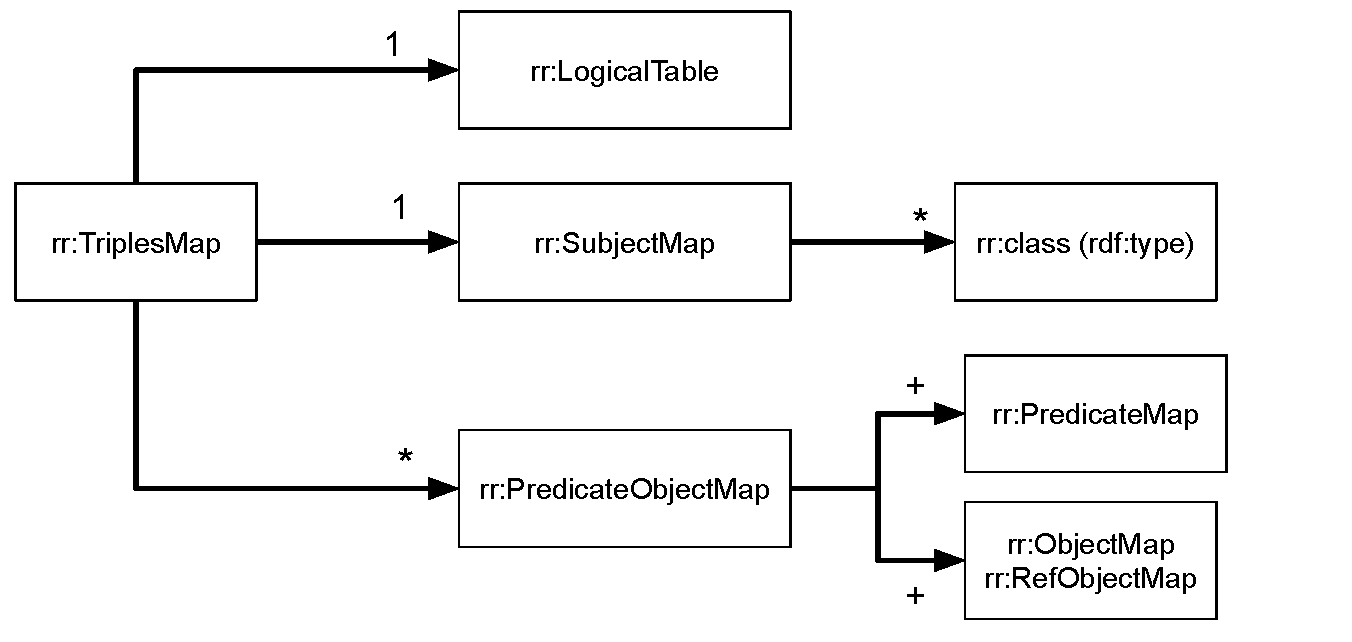
\includegraphics[width=\textwidth]{figures/state-of-the-art/R2RML-structure.pdf}
\caption{R2RML structure with its relevant properties~\citep{R2RML}}
\label{fig:soa_r2rml-structure}
\end{figure}

Figure \ref{fig:soa_r2rml-structure} shows the basic structure of an R2RML Triples Map, with the relations between its main properties and their cardinalities. \texttt{rr:SubjectMap}, \texttt{rr:PredicateMap} and \texttt{rr:ObjectMap} are defined as term maps (\texttt{rr:TermMap}. This property is used to generate the desirable RDF terms, either as IRIs (\texttt{rr:IRI}) Blank Nodes (\texttt{rr:BlankNode}) or literal (\texttt{rr:Literal}). The values of the term maps can be specified using the following properties: \texttt{rr:Constant} for constant values, \texttt{rr:Column} for values obtained directly from a column of a table or \texttt{rr:Template} for the ones that are a concatenation between a string and a column reference, for example, to generate subject IRIs. Furthermore, additional information can be provided such as the language of a literal, using the \texttt{rr:Language} property, or its corresponding datatype with \texttt{rr:Datatype}. Figure \ref{fig:soa_termmap-structure} gives an overview of the R2RML term map.


\begin{figure}[!t]
\centering
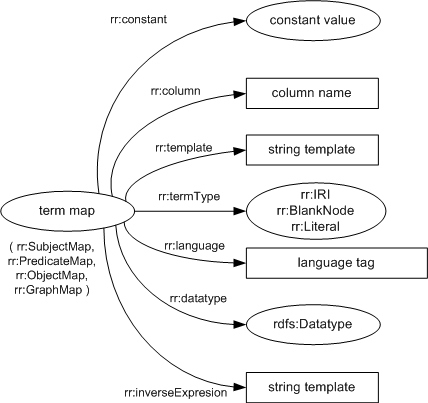
\includegraphics[width=0.7\textwidth]{figures/state-of-the-art/term-map.png}
\caption{R2RML \texttt{rr:TermMap} overview~\citep{R2RML}}
\label{fig:soa_termmap-structure}
\end{figure}

We provide a complete example of the construction of a knowledge graph through an R2RML mapping. The input table (Figure \ref{fig:soa_csv}) represents information about the stop times for a given trip of the Madrid's metro system. It provides the corresponding identifier for the trip and each stop together with the pickup time and type. Figure \ref{fig:soa_r2rml} shows the R2RML mapping for transforming the input table to a RDF dataset following the LinkedGTFS\footnote{\url{https://lov.linkeddata.es/dataset/lov/vocabs/gtfs}} ontology. We can observe that the subject map uses an \texttt{rr:template} with reference to three different columns of the table to generate unique identifiers for the IRIs. The set of \texttt{rr:PredicateObjectMap} (POM) defines the rules to generate three different properties of the \texttt{gtfs:StopTime} class. The \texttt{gtfs:arrivalTime} POM uses the \texttt{rr:dataType} property to declare the type of the input data, \texttt{gtfs:pickupType} uses the \texttt{rr:template} to generate an uri-based literal in the output dataset, and finally, \texttt{gtfs:trip} predicate has a \texttt{rr:RefObjectMap} to generate its corresponding object, referencing to the corresponding IRI trip defined in antoher TriplesMap. Finally, the output RDF dataset is shown in Figure \ref{fig:soa_rdf}.

\begin{figure}[!t]
\centering
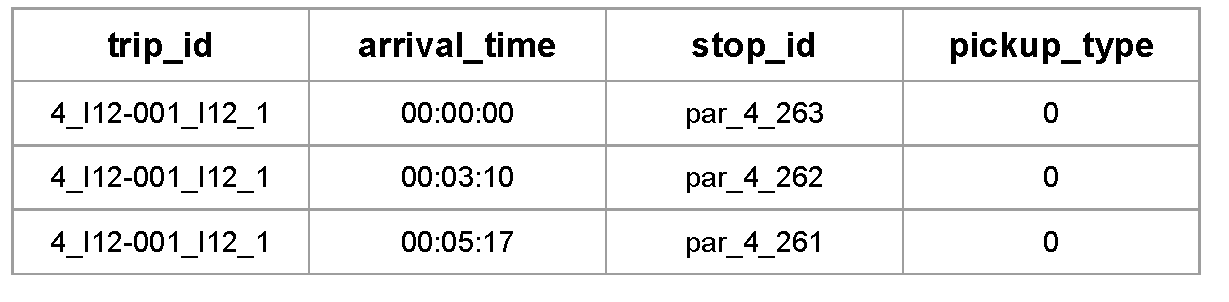
\includegraphics[width=0.85\textwidth]{figures/state-of-the-art/Stop_times CSV.pdf}
\caption{Excerpt of a Stop-times table}
\label{fig:soa_csv}
\end{figure}

\begin{figure}[!ht]
\centering
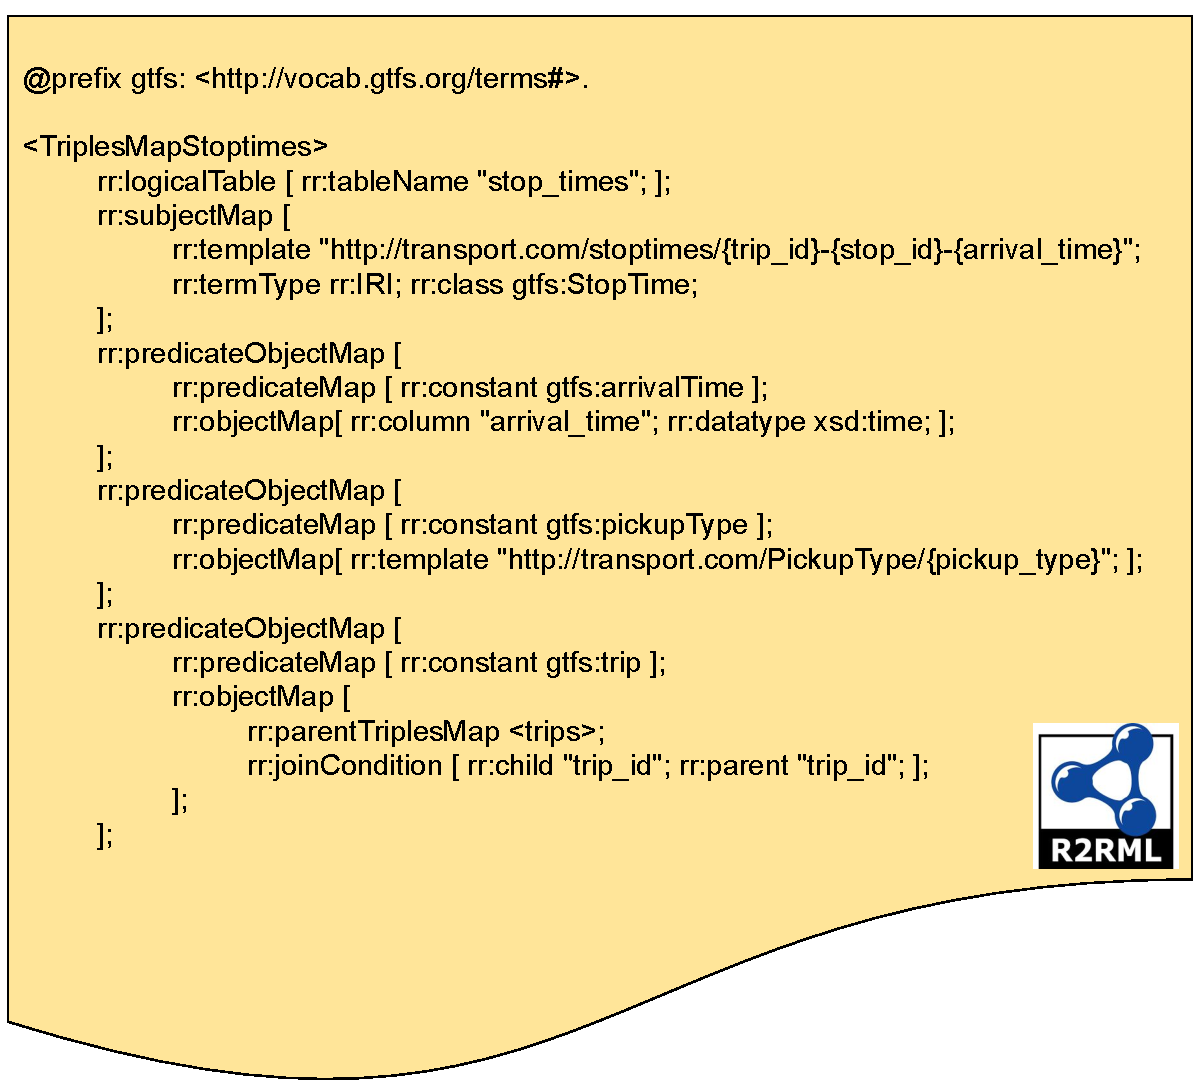
\includegraphics[width=0.85\textwidth]{figures/state-of-the-art/R2RML-example.pdf}
\caption{R2RML mapping for stop-times table}
\label{fig:soa_r2rml}
\end{figure}


\begin{figure}[!ht]
\centering
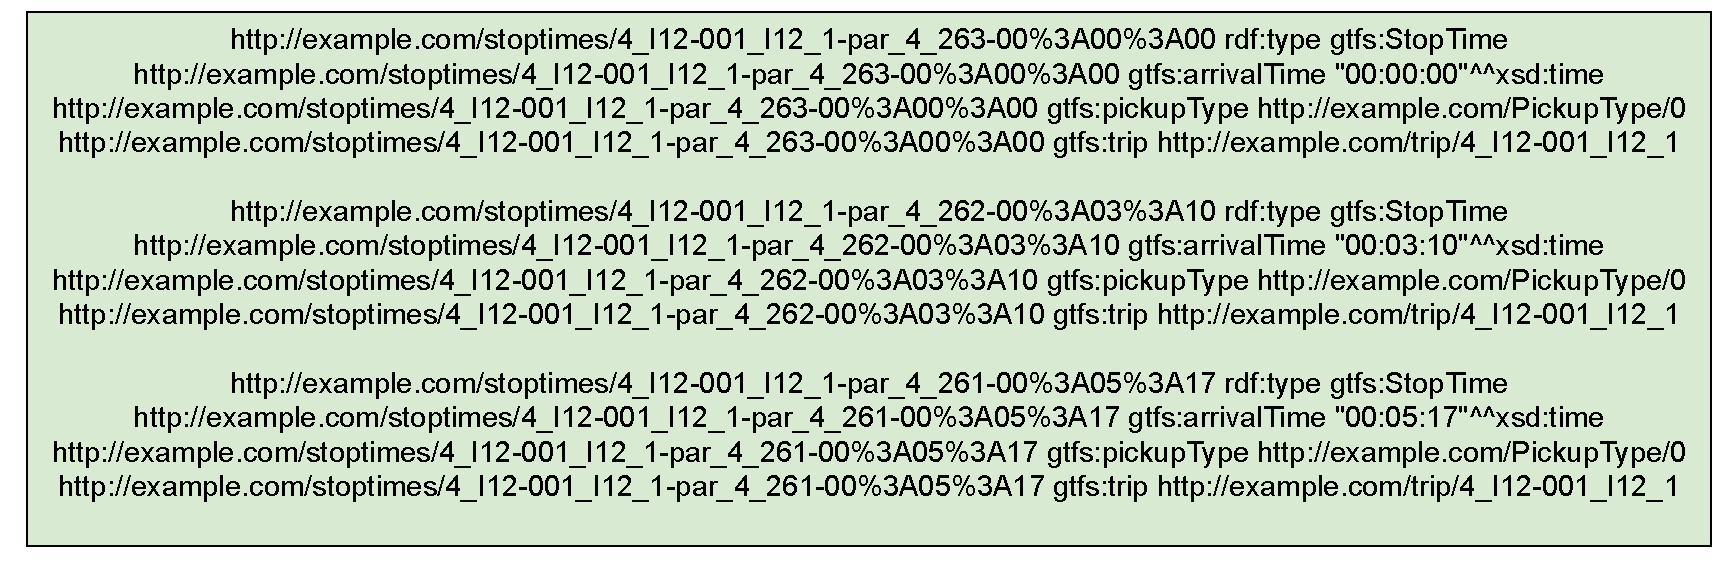
\includegraphics[width=0.85\textwidth]{figures/state-of-the-art/RDF from Stop_times.pdf}
\caption[RDF Generation from R2RML mapping rules]{Output RDF dataset after evaluating the R2RML document on the original data source}
\label{fig:soa_rdf}
\end{figure}



\subsubsection{RML: Extending R2RML for Heterogeneous Data}
The RDF Mapping Language (RML)~\citep{dimou2014rml} extends the R2RML mapping specification to cover other kinds of data formats such as CSV, XML or JSON, hence, this specification is one of the most used for constructing knowledge graph from heterogeneous data sources. In this section we explain the main differences between RML and R2RML and then we describe another serialization of the RML mappings following a YAML syntax, and its main properties~\citep{Heyvaert2018Declarative}.


\begin{table}[!t]
\centering
\caption{The differences between R2RML and RML~\citep{dimou2020high}}
\label{tab:soa_rmlvsr2rml}
\begin{tabular}{l|c|c}
                                          & \textbf{R2RML}                      & \textbf{RML}                         \\
\hline                                          
\textbf{Input reference}                  & Logical Table                       & Logical Source                       \\
\hline
\textbf{Data source language}             & SQL (implicit)                      & Reference Formulation (explicit)     \\
\hline
\multirow{2}{*}{\textbf{Value reference}} & \multirow{2}{*}{column}             & Logical reference \\
                                          &                                     & (valid expression acc. \\
                                          &                                     & Reference Formulation) \\
\hline                                          
\multirow{2}{*}{\textbf{Iteration}}       & \multirow{2}{*}{per row (implicit)} & per record        \\
                                          &                                     & (explicit -- valid expression        \\
                                          &                                     & acc. Reference Formulation)
\end{tabular}
\end{table}


\noindent Summarized in Table \ref{tab:soa_rmlvsr2rml}, the main differences between R2RML and RML are:

\noindent\textbf{{Logical Source.}} A Logical Source extends R2RML's Logical Table and describes the input data source used to generate the RDF. The Logical Table is only able to describe relational databases,whereas the Logical Source defines different heterogeneous data sources, including relational databases.

\noindent\textbf{{Reference Formulation.}} As RML is designed to support heterogeneous data sources. Data in a specific format can be parsed according to the grammar of a certain formulation (e.g., path and query languages or custom grammars). For example, one can refer to data in an XML file via XPath and in a relational database via SQL. To this end, the \emph{Reference Formulation} was introduced indicating the formulation used to refer to data in a certain data source.

\noindent\textbf{{Iterator.}} In R2RML processors iterate over each row to generate RDF. However, as RML is designed to support heterogeneous data sources, the iteration pattern cannot always be implicitly assumed. For example, iterating over a specific set of objects is done by selecting them via a JSONPath expression. To this end, the \emph{Iterator} was introduced which determines the iteration pattern over the data source and specifies the extract of data used to generate RDF during each iteration. The iterator is not required to be specified if there is no need to iterate over the input data.

\noindent\textbf{{Logical Reference.}} When referring to values in a table or view of a relational database, R2RML relies on column names. However, as RML is designed to support heterogeneous data sources, rules may also refer to elements and objects, such as in the case of XML and JSON. Consequently, references to values should be valid with respect to the used reference formulation. For example, a reference to an attribute of a JSON object should be a valid JSONPath expression. To this end, (i) the \verb|rml:reference| is introduced to replace \verb|rr:column|, (ii) when a template is used, via \verb|rr:template|, the values between the curly brackets should have an expression that is valid with respect to the used reference formulation, and (iii) \verb|rr:parent| and \verb|rr:child| of a Join Condition should also have an expression that is valid with respect to the used reference formulation.


YARRRML~\citep{Heyvaert2018Declarative} is a serialization of the RML mappings based on YAML syntax~\citep{ben2001yaml}. The aim of YARRRML is to help users in the creation of mapping rules using a human-readable approach. Figure \ref{fig:soa_yarrrml} shows an example of the mapping rules for constructing the KG based on the Stop Times CSV file show in Table \ref{fig:soa_csv}. The main keys used in a YARRRML-based mapping are \texttt{prefixes} to define the used prefixes and \texttt{mappings} where the rules are specified. Each \texttt{rr:TriplesMap} is defined with a key defined by the user (stoptimes in the example), and then three main keys have to be declared: \texttt{sources} for the input sources, \texttt{s} for generating the subject and then \texttt{po} for the \texttt{rr:PredicateObjectMap} properties. In the same manner as in [R2]RML, the defined identifier for the \texttt{rr:TriplesMap} is used for the \texttt{rr:RefObjectMap} declarations (e.g., trips in Figure \ref{fig:soa_yarrrml}). Additionally, this approach provides a translator to RML\footnote{\url{https://rml.io/yarrrml/matey/}}, so that any RML-compliant engine can be used when the rules are defined following this serialization.




\begin{figure}[!ht]
\centering
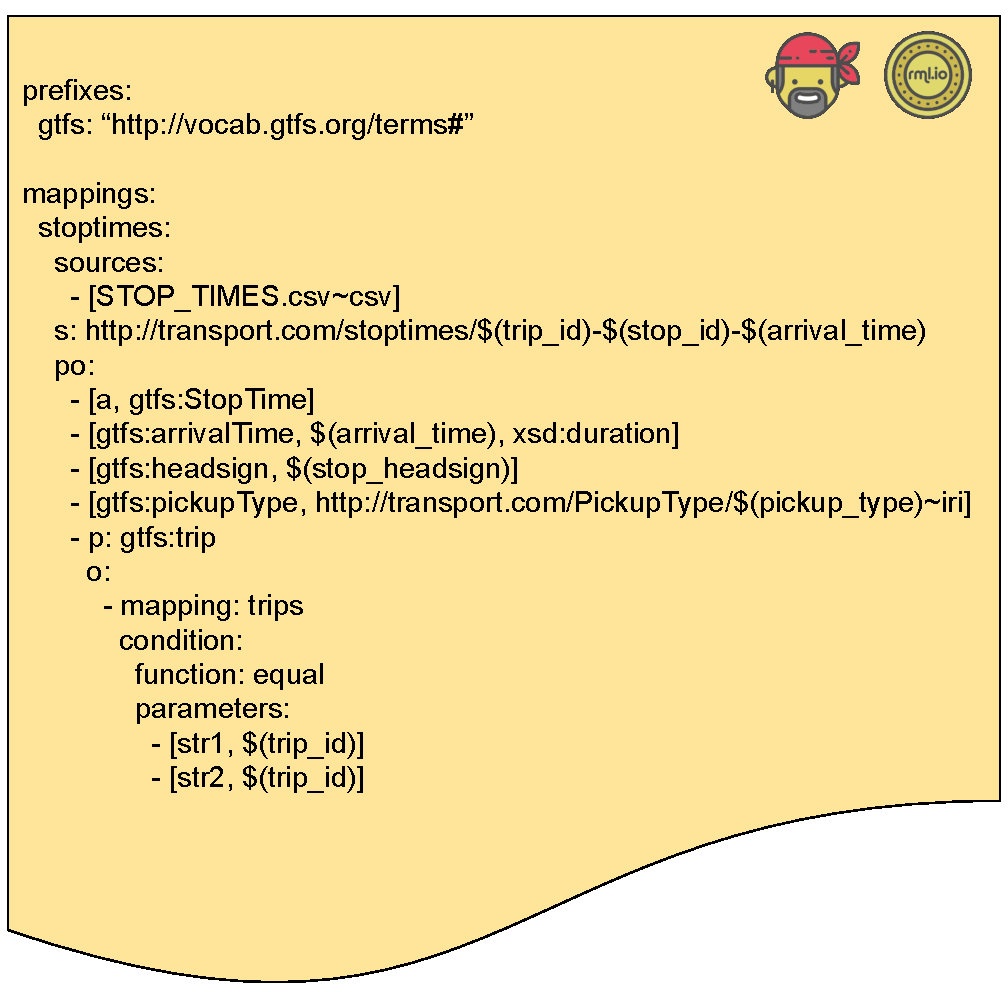
\includegraphics[width=0.7\textwidth]{figures/state-of-the-art/YARRRML example.pdf}
\caption{YARRML mapping example based for transforming Stop Times table}
\label{fig:soa_yarrrml}
\end{figure}

\subsubsection{Other approaches to Construct Knowledge Graphs}
There are a set of mapping languages and engines for constructing knowledge graphs that include special features. Instated of being a general solution to be applied in a declarative manner to any kind of data format, there are some proposals that focus on providing support to concrete issues that can appear in some data formats or extend other semantic web technologies for defining these rules such as SPARQL~\citep{SPARQL} or ShExML~\citep{prud2014shape}.  

\noindent\textbf{xR2RML.} The xR2RML proposal~\citep{michel2015translation} extends R2RML to describe mappings from NoSQL databases (e.g., MongoDB) to RDF. It also includes some of the properties from RML such as the \texttt{rml:iterator}. It contains three distinctive features to deal with issues that usually appear when hierarchical documents (XML or JSON) have to be mapped to an RDF model:
\begin{itemize}
    \item \textbf{Access to outer fields.} When a hierarchical structure has to parse to RDF, sometimes it is necessary to combine data from different levels of the tree. xR2RML incorporates the \texttt{xrr:pushDown} property with that aim. It allows the declaration of an external field outside the iterator defined, so it can be used in any part of the mapping. It is declared inside the logical source object with two properties. \texttt{xrr:reference} which defines the data reference of the value and \texttt{xrr:as} which declare the alias to be used within the mapping.  
    \item \textbf{Dynamic language tag.} xR2RML extends the \texttt{rr:language} property from R2RML and replaces it by \texttt{xrr:languageReference}. This property allows to define the language of an object dynamically, using a reference that can get the value from the database.
    \item \textbf{RDF lists and containers.} In formats such as JSON it is very common to have values that are modeled as arrays of data. This kind of data structures are also allowed in RDF using \texttt{rdfs:Container} with its corresponding subclasses \texttt{rdf:Bag}, \texttt{rdf:Seq} and \texttt{rdf:Alt} when there is not order, and the \texttt{rdf:List} class is used when there is an order. xR2RML extends the term map types including \texttt{xrr:RdfList}, \texttt{xrr:RdfBag}, \texttt{xrr:RdfSeq} and \texttt{xrr:RdfAlt} that allow the construction of these data structures in RDF.
\end{itemize}

\noindent\textbf{SPARQL-Generate.} The solution proposed in~\citep{lefranccois2017sparql} presents a template-based language to construct knowledge graphs extending SPARQL 1.1. It exploits the representation capabilities from SPARQL to declare the transformation rules inside the query. The approach of using SPARQL to define the transformation rules has been also proposed in previous approaches focused on specific data formats such as Tarql for CSV files\footnote{\url{https://tarql.github.io/}}. However, this kind of solution follows a procedural approach to define rules, instead of a declarative one. Therefore, and in comparison with the rest of proposals, they cannot exploit the benefits of declarative definition of rules such as the maintainability, reproducibility and understandability.

\noindent\textbf{ShExML.} In~\citep{garcia2020shexml}, the authors propose a solution based on the validation language for knowledge graphs, ShEx~\citep{prud2014shape}. Although it is based on this specification, it uses its own syntax and grammar. In comparison to R2RML-based proposals, ShExML separates the declaration, how to extract the data from the input sources, from the shapes, how to generate the desirable RDF graph. The main objective of this proposal is to help users to create the rules, and it also provides a translation engine to transform ShExML rules to RML mappings.


% Please add the following required packages to your document preamble:
% \usepackage{graphicx}
\begin{table}[t]
\centering
\caption{Summary of Mapping Languages specifications}
\label{tab:soa_sum_mappings}
\resizebox{0.85\textwidth}{!}{%
\begin{tabular}{|l|c|c|c|c|c|}
\hline
\textbf{Features/Mappings} & \textbf{R2RML} & \textbf{RML} & \textbf{xR2RML} & \textbf{SPARQ-Generate} & \textbf{ShExML} \\ \hline
Format & RDB & \begin{tabular}[c]{@{}c@{}}Heterogeneous\\ Datasources\end{tabular} & Tree-based formats & \begin{tabular}[c]{@{}c@{}}Heterogeneous\\ Datasources\end{tabular} & \begin{tabular}[c]{@{}c@{}}Heterogeneous\\ Datasources\end{tabular} \\ \hline
Type & Declarative & Declarative & Declarative & Procedural & Declarative \\ \hline
\begin{tabular}[c]{@{}l@{}}Special\\ Features\end{tabular} & \begin{tabular}[c]{@{}c@{}}W3C\\ Recommendation\end{tabular} & \begin{tabular}[c]{@{}c@{}}Integration with\\ CSVW and FnO\end{tabular} & \begin{tabular}[c]{@{}c@{}}Access outer fields\\ Dynamic Language\\ RDF Lists\end{tabular} & \begin{tabular}[c]{@{}c@{}}Native support for\\ streaming data\end{tabular} & - \\ \hline
Based on & - & RML & R2RML and RML & SPARQL & ShEx \\ \hline
\begin{tabular}[c]{@{}l@{}}Transformation\\ Functions\end{tabular} & - & \begin{tabular}[c]{@{}c@{}}Function \\ Ontology\end{tabular} & - & \begin{tabular}[c]{@{}c@{}}SPARQL \\ Functions\end{tabular} & - \\ \hline
\end{tabular}%
}
\end{table}


\subsection{Declarative Constraints: Transformation Functions and Metadata}
Data constraints play a key role during a data integration process~\citep{cali2002data}. They allow validating an input dataset $D$ against a schema $S$. Previous proposals of knowledge graph construction over relational database (OBDA) such as Morph-RDB~\citep{priyatna2014formalisation} and Ontop~\citep{calvanese2017ontop}, assume the existence of integrity constraints explicitly defined over the schema $S$ to propose their optimizations in SPARQL-to-SQL transformation processes. Additionally, mapping recommendations (i.e., R2RML) for RDB2RDF approaches declare that cleaning or preparation steps are not part of the KG construction process and they have to be performed before running it. However, during the construction of a KG from heterogeneous data sources, these data may not be normalized, and information about relationships or column/key names are not always descriptive or homogeneous, among other possible issues. Hence, data consumers are usually forced to apply ad-hoc or manual data wrangling processes to consume these kind of data. In order to try to avoid manual and not reproducible cleaning/preparation steps, there are a set of declarative proposals to allow the description of constraints over data on the web. Specifically, we will be focused on two different ways to declare constraints: extensions of mapping specifications for including the possibility to define transformation functions inside the mapping rules and metadata to describe data content on the web. 

\subsubsection{Transformation Functions in Mappings}
\label{soa2:functions}
Rahm and Do~\citep{rahm2000data} reported the relevance of data transformations expressed with functions during data curation and integration. Grounding on this statement, different approaches have been proposed for facilitating the definition of functions to enhance data curation (e.g., \citep{galhardas2001declarative,GuptaSKGTM12,raman2001potter}). Similarly, declarative languages have been proposed to allow for the definition of functions in the mappings. An approach independent of a specific implementation context is described in~\citep{demeester2019implementation}. It enables the description, publication and exploration of functions and instantiation of associated implementations. The proposed model is the so called Function Ontology~\citep{de2016ontology} and the publication method follows the Linked Data principles. It is used as an extension over RML mapping rules to allow declaring declaratively these transformation functions~\citep{de2017declarative}. More in detail, to integrate RML and FnO, the authors create a new type of term map \texttt{fnml:FunctionMap}. This new term map defines how a function has to be executed with its definition and parameters following the Function Ontology. The alignment between RML and FnO is possible as they are both declarative and described in RDF. Previous works related to this topic focus on developing ad-hoc and programmed functions. For example, R2RML-F~\citep{debruyne2016r2rml} and FunUL~\citep{junior2016funul,junior2016incorporating} allow using functions in the value of the \texttt{rr:objectMap} property, so as to modify the value of the cells from a relational database first (R2RML-F) and other kinds of formats after (FunUL). KR2RML~\citep{slepicka2015kr2rml}, used in Karma, extends R2RML by adding transformation functions in order to deal with nested values. OpenRefine enables such transformations with the usage of GREL functions, which can be used in its RDF extension. 


Figure \ref{fig:soa_yarrrml_fno} shows an example of the integration between the RML mapping language and the Function Ontology following the YARRRML specification. We can observe that the object of the predicate \texttt{gtfs:headsign} is defined as \texttt{fnml:FunctionMap} term map, where we declarative indicate the function that has to be executed (\texttt{grel:lowercase}), with its corresponding parameters. In this example, the function only needs one parameter that is the reference to the column \texttt{stop\_headsign} from the Stop\_Times input source. Listing \ref{list:soa_fno_example} depicts how the output RDF graph after the application of the RML+FnO, where the \texttt{grel:lowercase} function has been applied over the object value of \texttt{gtfs:headsign}.

\begin{figure}[!ht]
\centering
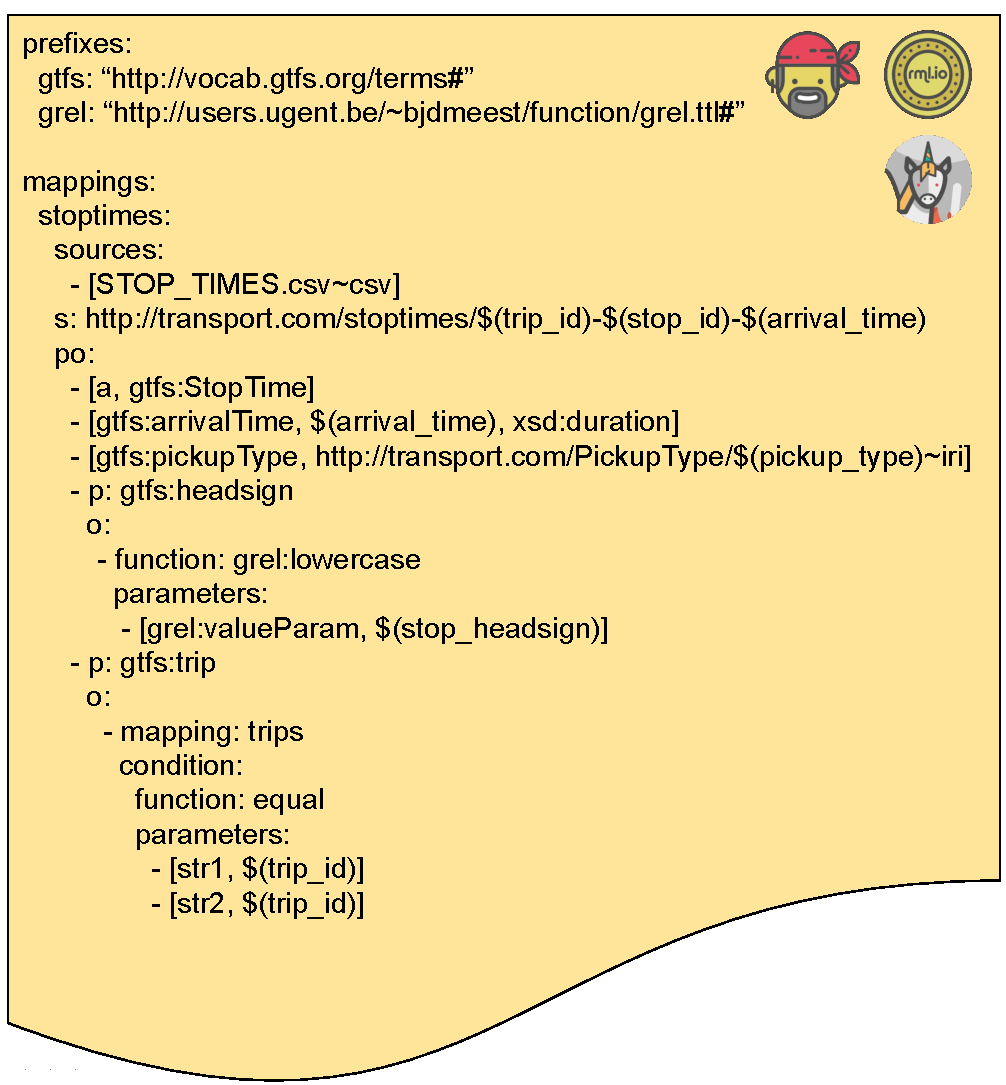
\includegraphics[width=0.7\textwidth]{figures/state-of-the-art/YARRRML+FnO.pdf}
\caption{YARRML mapping integrated with transformation functions following the FnO}
\label{fig:soa_yarrrml_fno}
\end{figure}


\begin{lstlisting}[float,caption=RDF graph generated by RML+FnO mapping,frame=tlrb,label={list:soa_fno_example}, columns=fullflexible]
@prefix gtfs: <http://vocab.gtfs.org/terms#> .
@prefix xsd: <http://www.w3.org/2001/XMLSchema#> .

<http://transport.org/trip/1> rdf:type gtfs:Trip .
<http://transport.org/trip/1> gtfs:stop <http://transport.org/stop/360> .
<http://transport.org/trip/1> gtfs:headsign ``puerta del sur'' .
<http://transport.org/trip/1> gtfs:wheelchair ``false''^^xsd:boolean .
\end{lstlisting}

\subsubsection{Metadata for data on the web}
Providing metadata for describing the content of a data source (e.g., data on the web) is a useful manner to obtain relevant information of a specific dataset that may be relevant during the construction of a knowledge graph. For example, DCAT~\citep{maali2018data} is a W3C recommendation to describe metadata from data catalogs. This standard is used, with some extension, in most of the open data portals across EU to describe the content of their datasets. Another relevant W3C recommendation for describing metadata is CSV on the Web~\citep{tennison2015model}.   
The recommendation\footnote{http://www.w3.org/TR/tabular-metadata/} defines a model for providing metadata on CSV files and other tabular data, such as datatypes, valid values, data transformations, and primary and foreign key constraints. A related W3C proposal\footnote{https://www.w3.org/TR/csv2rdf/} defines a procedure and rules for the generation of RDF from tabular data and a few implementations that refer to this proposal are already available such as COW\footnote{\url{https://csvw-converter.readthedocs.io/}}.

\begin{figure}[!ht]
\centering
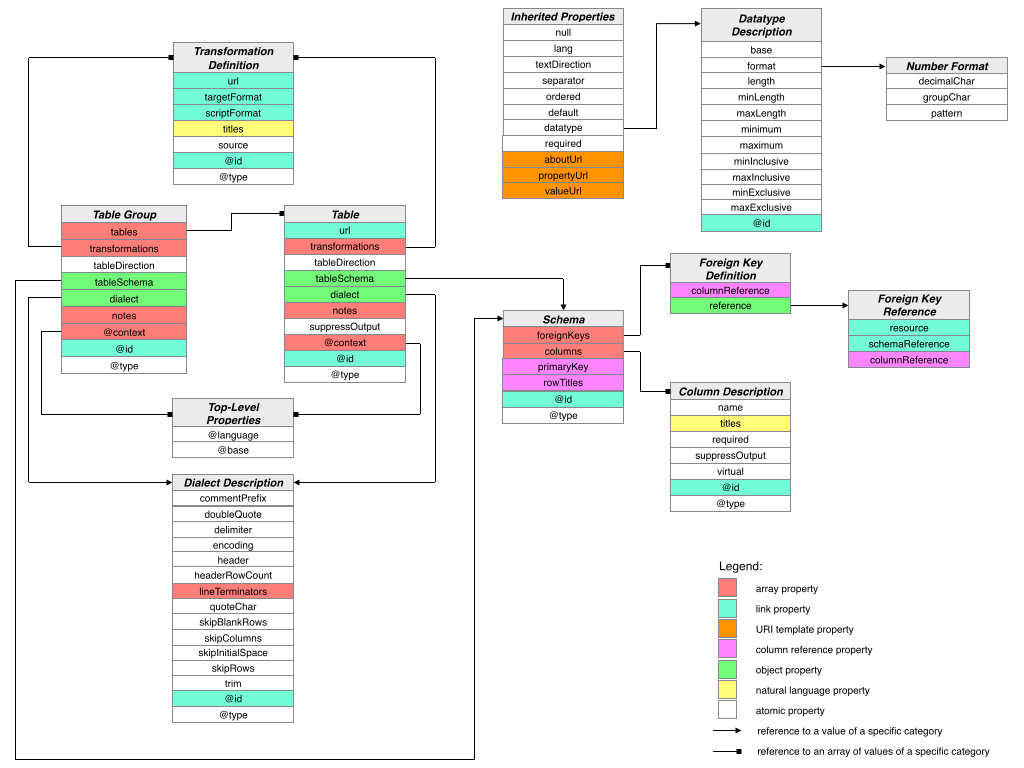
\includegraphics[width=0.85\textwidth]{figures/state-of-the-art/csvw-model.png}
\caption{The CSV on the Web model\citep{tennison2015model}}
\label{fig:soa_csvw}
\end{figure}


Taking into account this metadata during the process of KG construction from tabular datasets can help to enhance the process in terms of completeness and performance. It also allows dealing with the typical heterogeneity issues that appear in these kinds of data: data may not be normalized, information about relationships or column names are not always descriptive or homogeneous, missing (meta)data, etc. Figure \ref{fig:soa_csvw} shows the complete data model for describing tabular content on the web. It has been splinted in several parts that can describe the schema of the dataset, dialect annotations (e.g., delimiter value or the prefix used for comments) and information about datatype and related properties such as \texttt{csvw:null} (for null values) and \texttt{csvw:lang} (for the language). Each of these properties can be defined as an array, link, URI template, column reference or atomic value among others. The data model is materialized in a specific dialect of JSON-LD created for it, so that metadata annotations can be also expressed as an RDF graph, facilitating the interoperability of this proposal with others such as RML or R2RML. In Figure \ref{fig:soa_csvw_example} we show an example of CSVW annotations for our running example following the JSON-LD syntax. It provides useful information about the datatypes, column names or boolean values for the trips of a GTFS feed.

\begin{figure}[!ht]
\centering
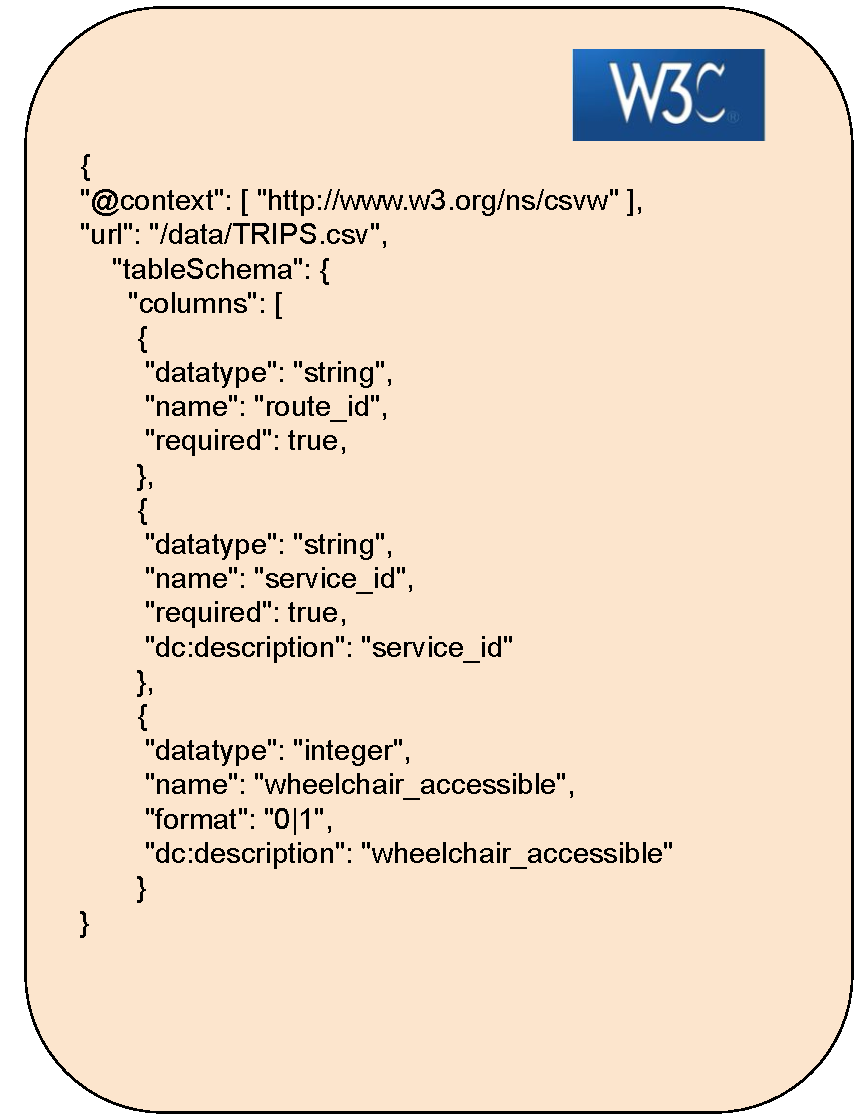
\includegraphics[width=0.5\textwidth]{figures/state-of-the-art/CVSW example.pdf}
\caption{An example of CSVW annotations over Transport Domain}
\label{fig:soa_csvw_example}
\end{figure}





\section{Knowledge Graph Construction Engines}
\label{sec:soa_engines}
Academic and industrial solutions for knowledge graph construction from structured and semi-structured data are gaining momentum. Since 2012, with the appearance of the W3C recommendation R2RML~\citep{R2RML}, diverse proposals, and optimization techniques have provided support for these transformations. We describe in detail engines for both groups of approaches, materialization and virtualization.

\subsection{Materialized Knowledge Graph Construction Engines}
With RML~\citep{dimou2014rml} proposed as an extension of R2RML for describing mapping rules over diverse data formats, multiple tools have been developed for the creation of knowledge graphs. There are multiple RML parsers\footnote{\url{https://rml.io/implementation-report/}}: CARML\footnote{\url{https://github.com/carml/carml}} executes RML rules and includes additional features like MultiTermMap (to deal with arrays) and XML namespace (to improve XPath expressions). RocketML~\citep{csimcsek2019rocketrml} is an RML engine implemented using the NodeJS framework that pre-processed join conditions to enhance the performance of the process. RMLMapper\footnote{\url{https://github.com/RMLio/rmlmapper-java}} is another RML engine implemented in Java and extensively used to obtain high-quality KGs. Additionally, RMLStreamer~\citep{haesendonck2019parallel} is an RML engine that is able to generate knowledge graphs from streaming data. There are other engines that are able to construct knowledge graphs from heterogeneous data sources without the support of mapping rules. For example, SPARQL-Generate~\citep{lefranccois2017sparql} is an engine based on SPARQL 1.1 that includes transformation rules within a SPARQL query. Chimera~\citep{scrocca2020turning} is based on RMLMapper and it includes a lowering step to convert RDF datasets into other formats and data models. Although most of the R2RML-compliant engines are able to generate materialized KGs from a RDB, their scientific contributions are focused on optimizations over the SPARQL-to-SQL process, so we describe them in the following section.

The CSV2RDF tool is presented in~\citep{Mahmud2018}, where the authors define algorithms to transform CSV data into RDF using CSVW metadata annotations, and their experimental study uses datasets from the CSVW Implementation Report\footnote{https://w3c.github.io/csvw/tests/reports/index.html}. Another tool, COW (Converter for CSV on the Web\footnote{https://csvw-converter.readthedocs.io/en/latest/}) allows the conversion of datasets in CSV format and uses a JSON schema expressed in an extended version of the CSVW recommendation. 

\subsection{Virtual Knowledge Graph Construction Engines}
Most of the works proposed under this framework are focused on providing access to relational databases~\citep{priyatna2014formalisation,calvanese2017ontop,sequeda2013ultrawrap} and optimizations on the  SPARQL-to-SQL translation process. The first approach on the translation between these two query languages is proposed in~\citep{chebotko2009semantics}, where the authors define an algorithm to create an equivalent SQL query based on an input SPARQL query. With the appearance of the R2RML recommendation, both Morph-RDB~\citep{priyatna2014formalisation} and Ontop~\citep{calvanese2017ontop} propose the use of these mapping rules and optimize the algorithm proposed in~\citep{chebotko2009semantics}. For example, there are recent studies and optimizations for an efficient translation of the \texttt{OPTIONAL} SPARQL operator in this process in~\citep{xiao2018efficient}. Nowadays, Morph-RDB and Ontop are the two most well known open source engines that construct virtual knowledge graph from relational databases. Ultrawrap~\citep{sequeda2013ultrawrap,sequeda2014obda} is another SPARQL-to-SQL engine that use SQL views to enhance the execution of the SQL queries after its translation from SPARQL. In~\citep{sequeda2014obda}, the authors propose a cost function that helps to decide when a SQL view should be or not physically materialize in the RDB.

In this context, the term constraint has been used in~\citep{hovland2016obda}, where the authors defined two new properties extending the concept of OBDA instance. They propose a set of optimizations during the SPARQL-to-SQL translation process with techniques that take into account these constraints. However, the main assumptions made over the OBDA framework (e.g, the data source is an RDB o has an RDB wrapper, or the schema contains a set of constraints) are maintained. There are other works such as~\citep{michel2015translation,botoeva2019ontology} that apply the OBDA framework over document-based databases. For example, in Morph-xR2RML~\citep{michel2015translation}, the authors formally define the translation from SPARQL to NoSQL databases.

There are two main proposals of the construction of virtual knowledge graphs beyond relational databases: Ontario and Squerall. Ontario~\citep{endris2019ontario} is based on the concept of RDF molecule templates~\citep{endris2017mulder} which aims to perform efficient source selection in a data lake composed of heterogeneous data sources in their original format. It creates a set of star-shaped sub-queries that match the RDF Molecule Templates (RDF-MT), and applies optimization techniques to define the query plan that will be executed. Similarly, Squerall~\citep{mami2019querying} takes input data and mappings, and offers a middleware that is able to aggregate the intermediate results in a distributed manner. Finally, Polyweb~\citep{khan2019one} is another proposal that is able to translate and distribute queries using RML mappings over relational databases and CSV files.



\section{Knowledge Graph Construction Evaluation Resources}
\label{sec:soa_evaluations}
To facilitate knowledge graph construction, KG engineers need to understand the strengths and weaknesses of the varied set of KGC engines that were presented in Section \ref{sec:soa_engines}. They may want to know whether their engines cover the requirements of their real-use-case scenarios. The challenge is to develop techniques and methodologies that cover the requirements for constructing knowledge graphs, and to ensure that is extensible and sustainable over time, when new approaches appear, or new versions of existing engines are released. In general, it is necessary to have an overview of state of the art engines that are tailored to different source formats, accepting as input those mappings that are represented in a variety of declarative languages. In this section we first provide an overview of test-cases defined to evaluate the conformance of KGC engines over a mapping language specification. Then we describe the main contributions about benchmark the performance and scalability of KGC engines.


\subsection{Test-Cases and Testbeds}
Whenever a specification becomes a W3C recommendation, such as SPARQL~\citep{SPARQL}, RDF~\citep{RDF}, Direct Mapping of relational data to RDF (DM)~\citep{directMapping}, and R2RML~\citep{R2RML}, several tools need to support them, and a set of test cases need to be defined for each of them (SPARQL test cases\footnote{ \url{https://www.w3.org/2001/sw/DataAccess/tests/r2}}, RDF 1.1 test cases\footnote{ \url{http://www.w3.org/TR/rdf11-testcases/}}, and R2RML and Direct Mapping test cases\footnote{\url{https://www.w3.org/TR/2012/NOTE-rdb2rdf-test-cases-20120814/}}). These test cases provide useful information to choose the tool that covers better certain needs. It is also a relevant step in the standardization process of any technology or specification. We describe the R2RML in more details as it is the one that is most related to the scope of our work.

Determining the conformance of tools executing R2RML rules in the process of RDF generation is a step to provide objective information about the features of each tool. For this reason, the R2RML test cases~\citep{R2RML_test_cases} were proposed, with 63 test cases. Each test case is identified by a set of features, such as the SQL statements to load the database, title, purpose, specification reference, review status, expected result, and corresponding R2RML rules. All the test cases are semantically described using the RDB2RDF-test\footnote{\url{http://purl.org/NET/rdb2rdf-test\#}} and Test Metadata Vocabulary\footnote{\url{https://www.w3.org/TR/2005/NOTE-test-metadata-20050914/}}. In 2021, several R2RML processors were assessed for their conformance with the R2RML specification running the test-cases. The results were available in the R2RML implementation-report~\citep{R2RML_implementation_report}, and are also annotated semantically using the Evaluation and Report Language (EARL) 1.0 Schema\footnote{\url{https://www.w3.org/TR/EARL10/}}.

%The Semantic Web community has also actively worked on the definition of several testbeds. As an example of the existing contributions, we can mention the work done in the area of federated query processing. Specifically in this area, FedBench~\citep{schmidt2011fedbench} is an exemplar benchmark; it comprises three datasets, (i.e. cross-domain, life science and SP$^2$Bench), 25 queries, and two proposed metrics to measure a federated engine performance, (i.e. total execution time and number of requests to SPARQL endpoints). LSLOD is another benchmark~\citep{hasnain2017biofed} that consists of 20 queries --classified as simple and complex; it comprises ten real-world datasets from the Life Sciences domain. LSLOD proposes to measure the performance in terms of total triple pattern-wise sources selected (TTPWSS), the number of SPARQL queries ASK, the source selection time, the overall query execution time, and the result set completeness. Finally,~\citep{montoya2012benchmarking} identify a main drawback in existing benchmarks for SPARQL federated queries; particularly, Montoya et al. focus on the study of FedBench and illustrate how the lack of considering independent variables impact on the effectiveness of the benchmark, e.g. complexity of the queries, data used, platforms involved, and endpoints. They show the relevance of these variables in order to ensure reproducibility of the results observed during an empirical evaluation. 

\subsection{Benchmarks}
\label{chap2:soa-bench}
Several benchmarks have been developed to measure the performance of SPARQL-to-SQL query translation of OBDA engines. The main two proposals in this field are the Berlin SPARQL Benchmark (BSBM)~\citep{bizer2009berlin} and the Norwegian Petroleum Directorate Benchmark (NPD)~\citep{lanti2015npd}. The BSBM benchmark sets its context in the e-commerce domain, and provides a configurable data generator and a set of SPARQL queries together with their equivalent SQL queries. This benchmark has been used to compare the query performance of native RDF stores with the performance of OBDA engines that execute virtualized SPARQL access against relational databases.

Specific OBDA requirements have been analyzed by the authors of the NPD benchmark in the setting of a real-world scenario from the oil industry. The nine proposed requirements are related to the datasets, query sets, mappings and query languages. The benchmark includes a data generator, VIG~\citep{lantivig}, to generate scaled RDB instances that obtain a number of expected triples from a SPARQL query, using as inputs an ontology, an R2RML mapping document, and the schema of the RDB together with its corresponding instance. 

Simple queries defined in LSLOD~\citep{hasnain2017biofed} have been used in order to evaluate the performance of the Ontario~\citep{endris2019ontario} engine. In this work, all of the original RDF datasets were translated into RDB tables. The idea was to evaluate an heterogeneous setup consisting of RDF and RDB sources, focused on the source selection problem, and the generation of the corresponding optimized query plan. Additionally, the simple queries from LSLOD are focused on the evaluation of the distribution of star-shaped groups that do not exploit some of the features of the SPARQL language, such as FILTER, ORDER BY, GROUP BY and NOT EXISTS, which are relevant in the context of  real-life use cases.

Many other benchmarks have been proposed in the Semantic Web area, but can be considered out of the scope of our work since they do not focus on KG construction. This includes for exmaple, FedBench~\citep{schmidt2011fedbench} and QFed~\citep{rakhmawati2014qfed} for SPARQL query federation or SP2Bench~\citep{schmidt2009sp} and HOBIT~\citep{roder2020hobbit} for RDF triplestores.

\section{Conclusions and limitations of the State of the Art}
\label{sec:soa_conclusions}
After the analysis and description of the state of the art in knowledge graph construction from heterogeneous data sources, we want to conclude this section with the identification of the strengths and weaknesses of the field that have motivated our work:
\begin{itemize}
    \item \textbf{Overlapping among mapping language specifications.} There are many mapping languages that allow defining rules for constructing knowledge graphs from heterogeneous data sources. Although they usually have their own specific features for solving different problems, they also share multiple features. Languages are not necessarily interoperable, and many of them come associated with a very specific engine that supports them. Having the possibility of translating among these different languages would allow practitioners to have the possibility of selecting a wider set of engines to implement their knowledge graph construction process.
    \item \textbf{The importance of declarative approaches.} The use of declarative and standardized mapping rules and metadata makes it possible to generalize a proposal, avoiding ad-hoc and manual steps. It also incorporates a set of important benefits for a KG construction process, such as the improvement of its maintainability, reproducibility readability, and understandability.
    \item \textbf{Constructing virtual KG over heterogeneous data sources.} Most of the data shared on the web is currently raw data in well known formats such as CSV, JSON, and XML. Semantic Web and more specifically, KG construction technologies, play a key role in starting to see the web as an integrated  database that can be queried. Querying heterogeneous and flat data is: i) neither a trivial nor an easy task that can be delegated to na\"ive querying approaches and ii) optimizations and improvements can still be proposed taking advantage and exploiting current annotation proposals to not only enhance performance but also completeness. Most of the virtual knowledge graphs construction engines over heterogeneous data sources have focused on the adaptation of techniques proposed by federated SPARQL engines, but they do not support the majority of the SPARQL operators and they do not correctly execute the queries when the data source is beyond RDB instances.
    \item \textbf{Constructing materialized KGs at scale.} Despite the rich repertory of knowledge graph construction approaches using materialization techniques, optimizing the declarative description of complex data integration systems (i.e., heterogeneous data sources, high rate of duplicates, application of transformation functions, big data sizes, etc.) remains still open. The absence of frameworks capable of efficiently executing complex data integration systems negatively impacts on the global adoption of existing formalisms in real-world applications of knowledge graphs.
    \item \textbf{Comprehensive evaluations KG construction approaches.} The absence of testbeds, test-cases and benchmarks for knowledge graph construction has prevented the community from conducting fair evaluations of the existing engines. This resource deficiency has also impeded for a holistic understanding about the pros and cons of the state of the art, as well as for clear directions to advance the area. Given the expected growth rate of available data, these evaluation standard methodologies are demanded in order to devise the next generation of tools able to integrate data at scale.
\end{itemize}